\chapter{Results}
\label{sec:results}


%%%%%%%%%%%%%%%%%%%%%%%%%%%%%%%%%%%%%%%%%%%%%%%%%%%%
\section{Architecture selection on clean sounds}
\label{sec:results:clean}

For the architecture selection, we use random search as described in section~\ref{methods:architecture:random}. Several architectures can thus be tested and their relative performances compared. The metrics we used are the test accuracy (in mean and maximum), the test loss (in mean) and the test-train difference (in relative difference). For the architecture selection, we favored identification over localization as localization is proved easier to learn as seen in section~\ref{sec:results:multi}.

The tested architectures are presented on table~\ref{fig:results:clean_table} and compared on figures~\ref{fig:results:max_test_accuracy}~to~\ref{fig:results:test_train_diff}.

\renewcommand{\arraystretch}{1.5}
\begin{table}[htb]
\begin{tabular}{|p{.25\textwidth}|p{.75\textwidth}|}
\hline
\verb+rmp_1conv_2ip+ & Using only ratemaps, one convolutional stage followed by two inner products \\
\hline
\verb+rmp_2conv_1ip+ & Using only ratemaps, two convolutional stages followed by one inner product \\
\hline
\verb+rmp_2conv_2ip+ & Using only ratemaps, two convolutional stages followed by two inner products \\
\hline
\verb+rmp_3conv_1ip+ & Using only ratemaps, three convolutional stages followed by one inner product \\
\hline
\verb+ams_1conv_2ip+ & Using only AMS, one convolutional stage followed by two inner products \\
\hline
\verb+amsrmp_2conv_2ip+ & Using all available features (AMS and ratemaps), two convolutional stages followed by two inner products \\
\hline
\verb+amsrmp_2conv_2ip+ & Using AMS and ratemaps, two convolutional stages followed by two inner products \\
\hline
\verb+amsrmp_2dconv_1ip+ & Using AMS and ratemaps, two parallel convolutional stages for both features followed by a concatenation stage and one single inner product; the models learn different weights for the two convolutions; the parameters of the convolution however are the same, so that they produce outputs of the same size that can be concatenated \\
\hline
\end{tabular}
\\
\caption{Tested architectures for clean sounds}
\label{fig:results:clean_table}
\end{table}

\begin{figure}[htb]
\label{fig:results:clean}
\begin{subfigure}[t]{0.5\textwidth}
	\centering
	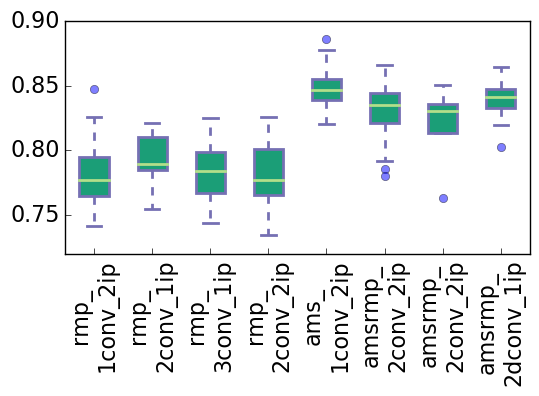
\includegraphics[scale=0.5]{images-architecture-clean/max_test_accuracy}
    \caption{Test accuracy in maximum}
	\label{fig:results:max_test_accuracy}
\end{subfigure}%
\begin{subfigure}[t]{0.5\textwidth}
	\centering
	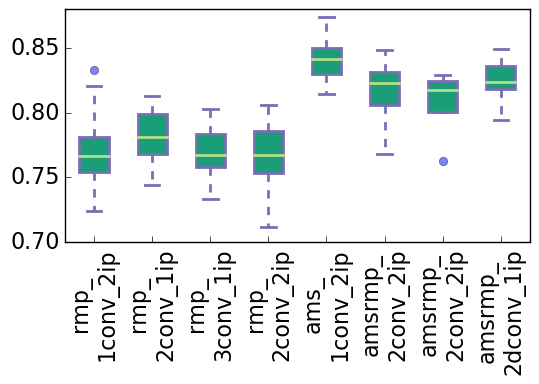
\includegraphics[scale=0.5]{images-architecture-clean/mean_test_accuracy}
    \caption{Test accuracy in mean}
	\label{fig:results:mean_test_accuracy}
\end{subfigure}
\begin{subfigure}[t]{0.5\textwidth}
	\centering
	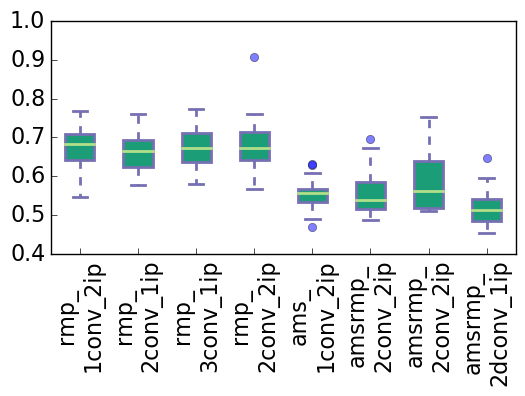
\includegraphics[scale=0.5]{images-architecture-clean/mean_test_loss}
    \caption{Test loss in mean on final plateau}
	\label{fig:results:mean_test_loss}
\end{subfigure}%
\begin{subfigure}[t]{0.5\textwidth}
	\centering
	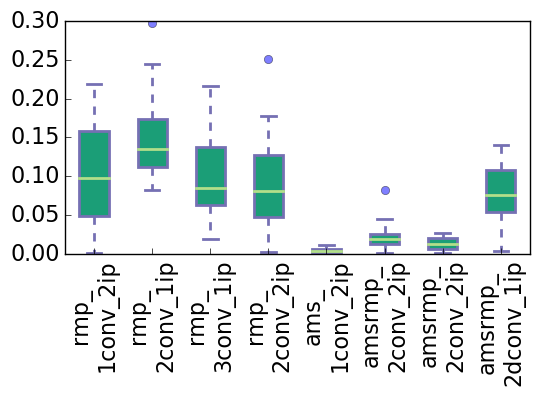
\includegraphics[scale=0.5]{images-architecture-clean/test_train_diff}
    \caption{Test-train difference}
	\label{fig:results:test_train_diff}
\end{subfigure}
\caption{Architecture selection results for clean sounds using several features and depths}
\end{figure}
The architecture using only AMS with one convolutional stage and two inner products (\verb+ams_1conv_2ip+) clearly stands out for all metrics with an accuracy mean of 87.4\% for identification.


%%%%%%%%%%%%%%%%%%%%%%%%%%%%%%%%%%%%%%%%%%%%%%%%%%%%
\section{Multitask learning on clean sounds}
\label{sec:results:multi}

We here intend to compare the learning speed and final performance of different multitask learning techniques, based on the same best model of section~\ref{sec:results:clean}. The tested architectures are presented on table~\ref{fig:results:multitask} and compared on figures~\ref{fig:results:id_test_accuracy} to~\ref{fig:results:loc_train_loss}.

\renewcommand{\arraystretch}{1.5}
\begin{table}[htb]
\begin{tabular}{|p{.15\textwidth}|p{.85\textwidth}|}
\hline
\verb+Id, loc+ & Sequential multitask learning starting with identification before learning both tasks \\
\hline
\verb+Loc, id+ & Sequential multitask learning starting with localization before learning both tasks \\
\hline
\verb+Joint+ & Joint multitask learning with all branches in common; only the output layers are task-specific; both losses have the same weight and are simultaneously optimized \\
\hline
\verb+Joint, sep+ & Joint multitask learning with the last layers optimized simultaneously, but separately (i.e. with different learnt weights) \\
\hline
\end{tabular}
\\
\caption{Tested architectures for multitask learning}
\label{fig:results:multitask}
\end{table}

All experiments were launched with the same training and testing parameters, so they can be properly compared. We took a moving average of the training loss on the last $30$ iterations, in order to smooth the learning curve and extract the global pattern.

\begin{figure}[htb]
\begin{subfigure}[t]{0.5\textwidth}
	\centering
	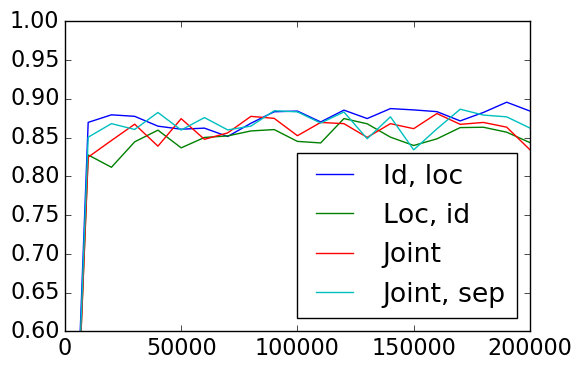
\includegraphics[scale=0.45]{images-architecture-compare/id_test_accuracy}
    \caption{Identification test accuracy}
	\label{fig:results:id_test_accuracy}
\end{subfigure}%
\begin{subfigure}[t]{0.5\textwidth}
	\centering
	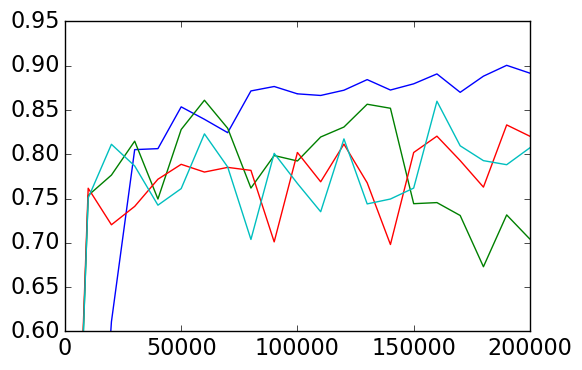
\includegraphics[scale=0.45]{images-architecture-compare/loc_test_accuracy}
    \caption{Localization test accuracy}
	\label{fig:results:loc_test_accuracy}
\end{subfigure}
\begin{subfigure}[t]{0.5\textwidth}
	\centering
	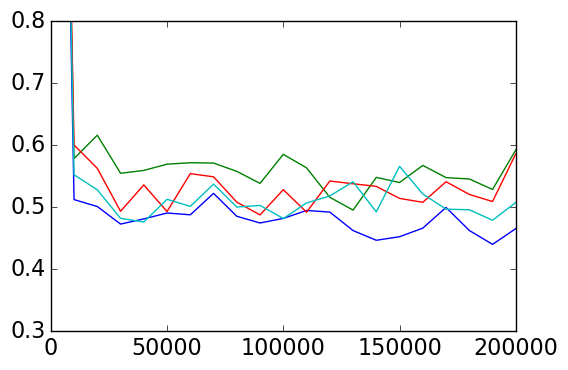
\includegraphics[scale=0.45]{images-architecture-compare/id_test_loss}
    \caption{Identification test loss}
	\label{fig:results:id_test_loss}
\end{subfigure}%
\begin{subfigure}[t]{0.5\textwidth}
	\centering
	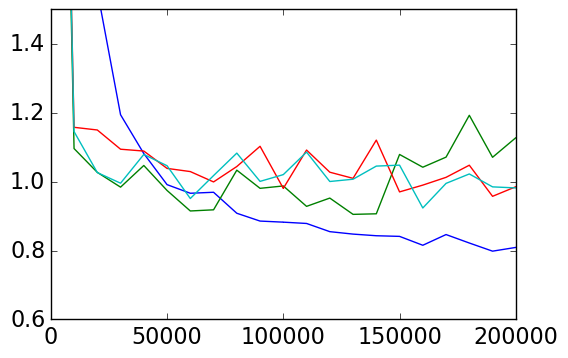
\includegraphics[scale=0.45]{images-architecture-compare/loc_test_loss}
    \caption{Localization test loss}
	\label{fig:results:loc_test_loss}
\end{subfigure}
\begin{subfigure}[t]{0.5\textwidth}
	\centering
	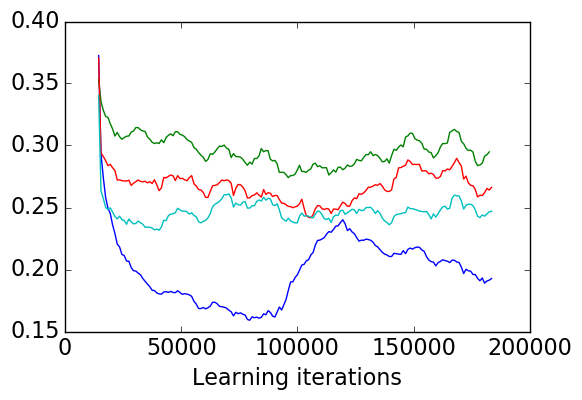
\includegraphics[scale=0.45]{images-architecture-compare/id_train_loss}
    \caption{Averaged identification train loss}
	\label{fig:results:id_train_loss}
\end{subfigure}%
\begin{subfigure}[t]{0.45\textwidth}
	\centering
    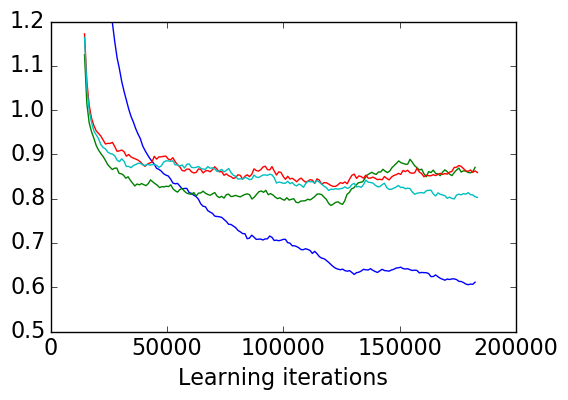
\includegraphics[scale=0.45]{images-architecture-compare/loc_train_loss}
    \caption{Averaged localization train loss}
    \label{fig:results:loc_train_loss}
\end{subfigure}
\caption{Learning curves with different multitask learning techniques for both tasks (identification on the left, localization on the right)}
\end{figure}

First of all, the convergence speeds to the desired plateau accuracies in \ref{fig:results:id_test_accuracy} and \ref{fig:results:loc_test_accuracy} confirm that identification is easier to learn for the network than localization.
We also notice that fine-tuning for multitask learning beginning with identification (i.e. the "easiest" task in terms of learning) seems more efficient, in that its test accuracy (the blue line in \ref{fig:results:id_test_accuracy} and \ref{fig:results:loc_test_accuracy}) converges much faster to the optimal accuracy for the desired tasks. Using fine-tuning would also allow to prioritize one task over another, in particularly by decreasing the learning rate or increasing the momentum after having trained one task. The second task to be trained will take some time to adjust as seen in \ref{fig:results:id_train_loss} and \ref{fig:results:loc_train_loss}. We finally achieve best plateau accuracies (best mean on the last 20\% plateau of the accuracy function) of 88.8\% for identification and 88.7\% for localization.

Secondly, for both identification and localization, there is a difference in the learning speed between the joint learning and the joint learning on separate branches as seen on \ref{fig:results:id_train_loss} and \ref{fig:results:loc_train_loss}. In mean, the training loss using full joint learning is 9\% higher than the training loss using separate branches for identification, and 5\% higher for localization. This means that the last layers of a CNN would construct features that are less transferable than early layers. As \citeauthor{yosinski2014transferable} \parencite{yosinski2014transferable} also argue, this supports the fact that first-layer features are general while last-layer features are more specific to the trained task. However, in our case, further experiments should be led with various architectures, in order to draw more general conclusions. In particularly, this phenomenon should be proved to be independent from the weight and bias initializations, which are currently set to random in all our experiments, as customary in deep learning. In that matter, averaging results on several learning and test phases can lead to more robust results.


%%%%%%%%%%%%%%%%%%%%%%%%%%%%%%%%%%%%%%%%%%%%%%%%%%%%
\section{Architecture selection on mixed sounds}
\label{sec:results:mixed}

As for mixed sounds, we also use random search as described in section~\ref{methods:architecture:random}. We did not rely on the architectures we found for clean sounds, as the data, the features and the complexity of the problem are all very different. The several models are compared by their test losses (in mean) and test-train loss differences (in relative difference), as other metrics require more expensive computations which are not compatible with random search.

The tested architectures are presented on table~\ref{fig:results:mixed_table} and compared on figures~\ref{fig:results:mean_test_loss_mixed} ~and~\ref{fig:results:test_train_diff_mixed}.
\renewcommand{\arraystretch}{1.5}
\begin{table}[htb]
\begin{tabular}{|p{.25\textwidth}|p{.75\textwidth}|}
\hline
\verb+ild_1conv2ip+ & Using ILD features only, one convolutional stage followed by two inner products \tabularnewline
\hline
\verb+all_1conv2ip_10x10+ & Using all available features (AMS, ILD and ratemaps), one convolutional stage followed by two inner products; the first convolutions are adjusted so that it produces outputs of the same size $10\times10$ for each feature, which can then be concatenated and fed into the inner products \tabularnewline
\hline
\verb+all_1conv2ip_12x16+ & With all features, one convolutional stage followed by two inner products; the first convolution outputs features of size $12\times16$ \tabularnewline
\hline
\verb+all_1conv2ip_16x16+ & With all features, one convolutional stage followed by two inner products; the first convolutions output features of size $16\times16$ \tabularnewline
\hline
\verb+all_2conv2ip_16x16+ & With all features, two convolutional stages followed by two inner products; the first convolution is as described above \tabularnewline
\hline
\verb+all_3conv2ip_16x16+ & With all features, three convolutional stages followed by two inner products; the first convolution is as described above \\
\hline
\end{tabular}
\\
\caption{Tested architectures for mixed sounds}
\label{fig:results:mixed_table}
\end{table}
\begin{figure}[htb]
\begin{subfigure}[t]{0.5\textwidth}
	\centering
	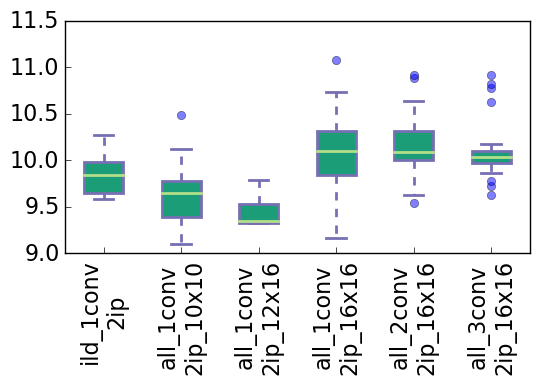
\includegraphics[scale=0.5]{images-architecture-mixed/mean_test_loss}
    \caption{Test loss in mean on final plateau}
	\label{fig:results:mean_test_loss_mixed}
\end{subfigure}%
\begin{subfigure}[t]{0.5\textwidth}
	\centering
	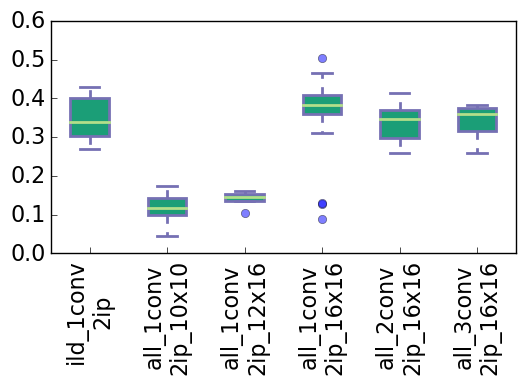
\includegraphics[scale=0.5]{images-architecture-mixed/test_train_diff}
    \caption{Test-train difference}
	\label{fig:results:test_train_diff_mixed}
\end{subfigure}
\caption{Architecture selection results for mixed sounds using several features and depths}
\end{figure}
We first tested each feature taken individually (results using only ratemaps and only AMS are relatively too poor to appear on the figures), then all features with architectures of increasing depths. As features have different sizes, the first convolutions are arranged to output features of same sizes that can then be processed in the rest of the network. For this purpose, we exploit the relationship in a convolution between the output size $W_{\text{ouput}}$, the input size $W_{\text{input}}$, the size $F$ of the convolution filter, the stride $S$ and the padding $P$ with which they are applied:
\begin{equation}
W_{\text{output}} = \frac{W_{\text{input}} - F + 2P}{S + 1}
\end{equation}

In this case, the test-train difference makes less sense because random search does not allow to train long enough to make training and test losses comparable. We retain three architectures with the three best test losses (\verb+all_1conv2ip_16x16+, \verb+all_2conv2ip_16x16+ and \verb+all_3conv2ip_16x16+).


%%%%%%%%%%%%%%%%%%%%%%%%%%%%%%%%%%%%%%%%%%%%%%%%%%%%
\section{Multitask learning performances on mixed sounds}
\label{sec:results:perf}

The best performing model from section~\ref{sec:results:mixed} is picked to be assessed using the specific metrics of section~\ref{sec:methods:metrics} (Evaluation metrics).

The best-identified classes by increasing order of ROC AUC are as shown on figure~3.4:
dog (0.778 ROC AUC),
female and male screams (0.763),
female speech (0.733),
knock (0.731),
male speech (0.723),
baby (0.709),
engine (0.706),
piano (0.702),
alarm (0.67),
fire (0.662),
phone (0.638),
footsteps (0.635) and
crash (0.609).

\begin{figure}
\hspace*{-2cm}
\centering
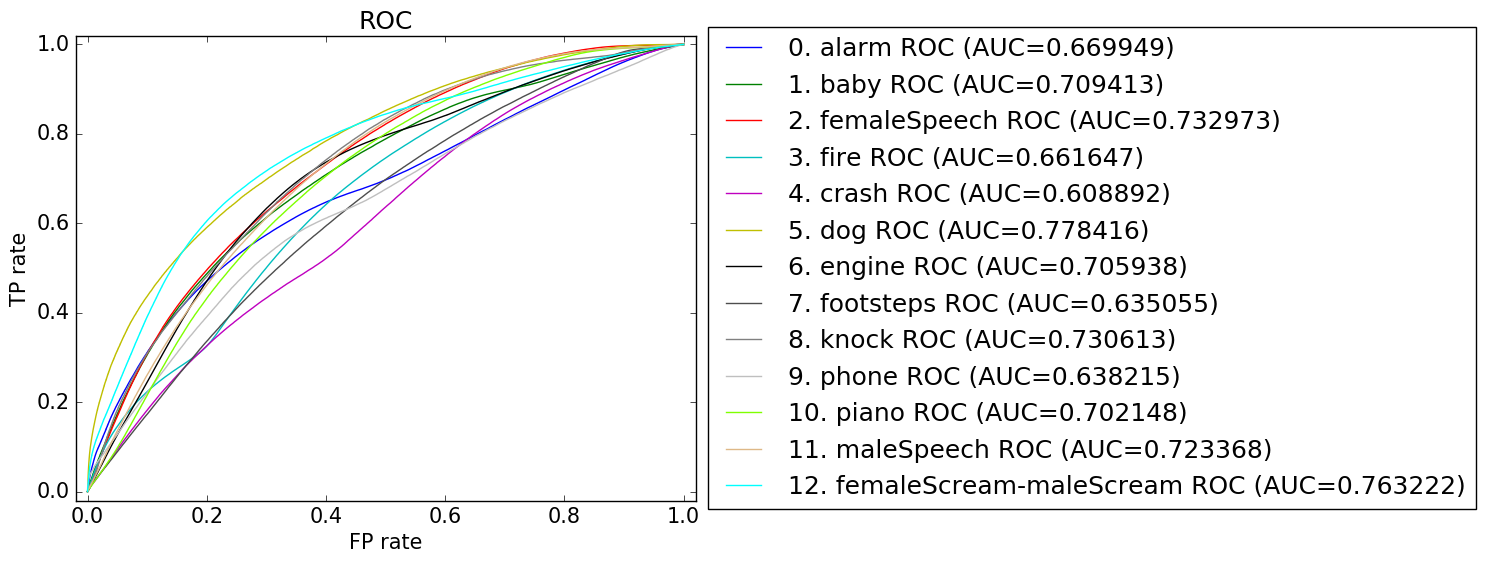
\includegraphics[scale=0.45]{images-architecture-mixed/id_roc}
\label{fig:results:id_roc}
\caption{Area under the curve of the receiving operating curve (AUC ROC) for identification classes}
\end{figure}

The maximal balanced accuracy calculated at the best classifier threshold also gives similar results as shown on figure~3.5:
female and male screams (70.95\% balanced accuracy),
dog (69.99\%),
knock (67.13\%),
engine (67.1\%),
male speech (66.71\%),
female speech (66.59\%),
baby (65.7\%),
piano (65.36\%),
alarm (63.88\%),
fire (62.4\%),
phone (61.5\%),
footsteps (59.93\%) and
crash (57.56\%). With both metrics, screams are the best-identified class.

\begin{figure}
	\hspace*{-4cm}
	\centering
	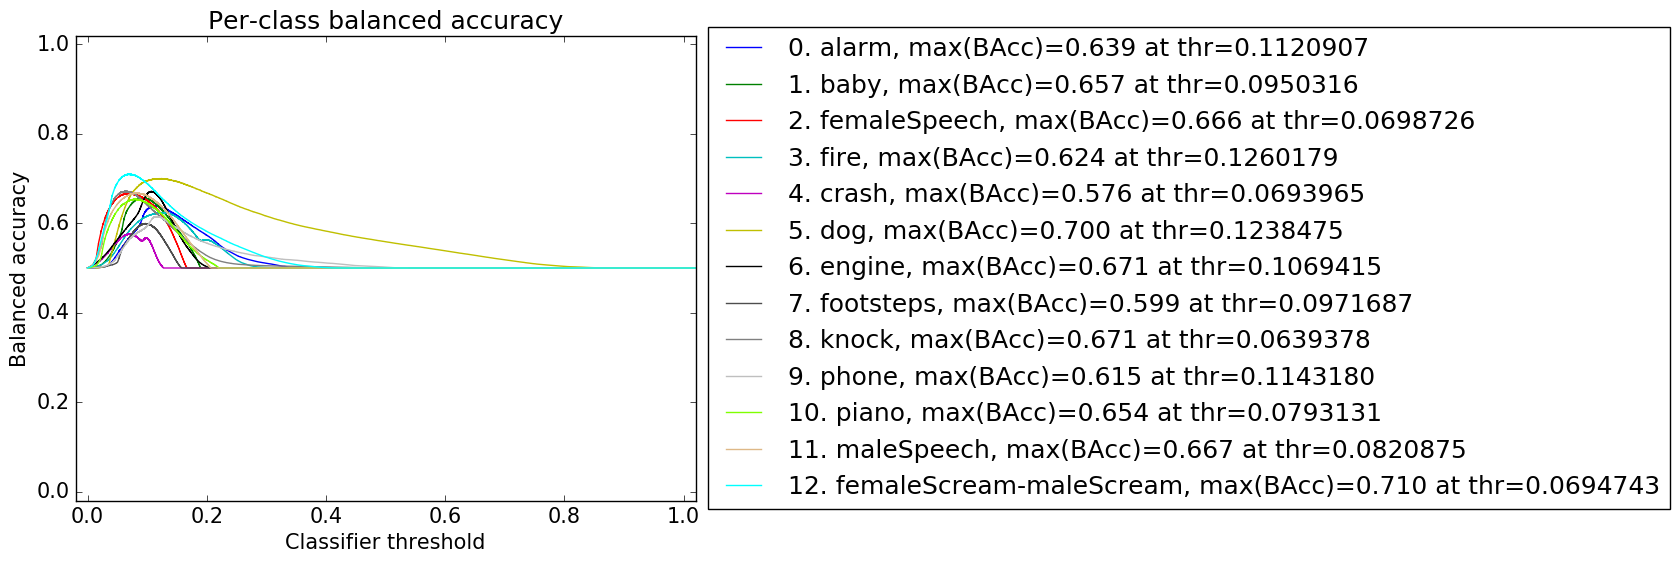
\includegraphics[scale=0.45]{images-architecture-mixed/id_max_bacc}
	\label{fig:results:id_max_bacc}
\caption{Identification classes balanced accuracy calculated for each classifier threshold}
\end{figure}

As for localization, balanced accuracy clearly indicates that the agent only achieves a near-chance performance, averaging at 53.15\% balanced accuracy, as shown in figure~3.6a. However the best-localized classes are:
-160.0$^\circ$ (60.05\% balanced accuracy),
-150.0$^\circ$ (59.23\%),
-100.0$^\circ$ (57.93\%),
-65.0$^\circ$ (56.66\%),
-90.0$^\circ$ (56.29\%),
-105.0$^\circ$ (55.63\%),
-180.0$^\circ$ (55.39\%),
-170.0$^\circ$ (55.23\%),
-140.0$^\circ$ (54.9\%) and
-130.0$^\circ$ (54.07\%).
However, figure~3.6b implies there is a correlation between the frequency of apparition of the azimuth in the training set and the obtained balanced accuracy for the corresponding azimuth. The dataset imbalance in terms of localization classes (as seen on figure~2.3c of section~\ref{sec:methods:balancing}) thus seems to penalize under-representated classes. Sufficient amounts of data is indeed essential for CNN to perform well and that can explain the gap between some localization classes. \\

\begin{figure}[htb]
\begin{subfigure}[t]{0.5\textwidth}
\hspace*{-1cm}
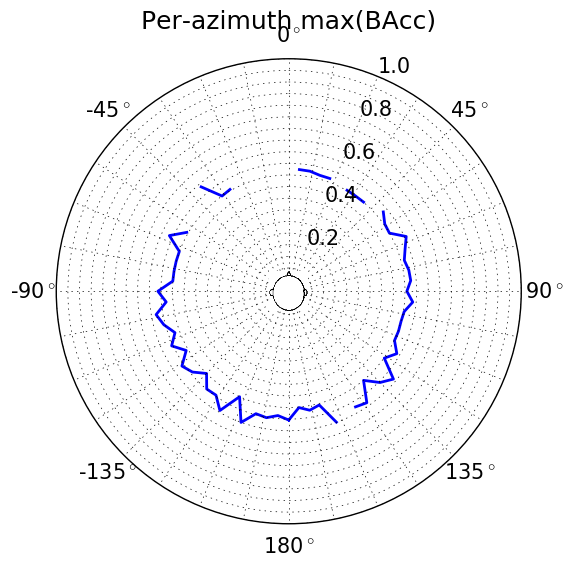
\includegraphics[scale=0.45]{images-architecture-mixed/loc_max_bacc}
\vspace*{.5cm}
\label{fig:results:loc_max_bacc}
\caption{Maximal balanced accuracy at best \\ classifier threshold for localization \\ classes}
\end{subfigure}
\begin{subfigure}[t]{0.5\textwidth}
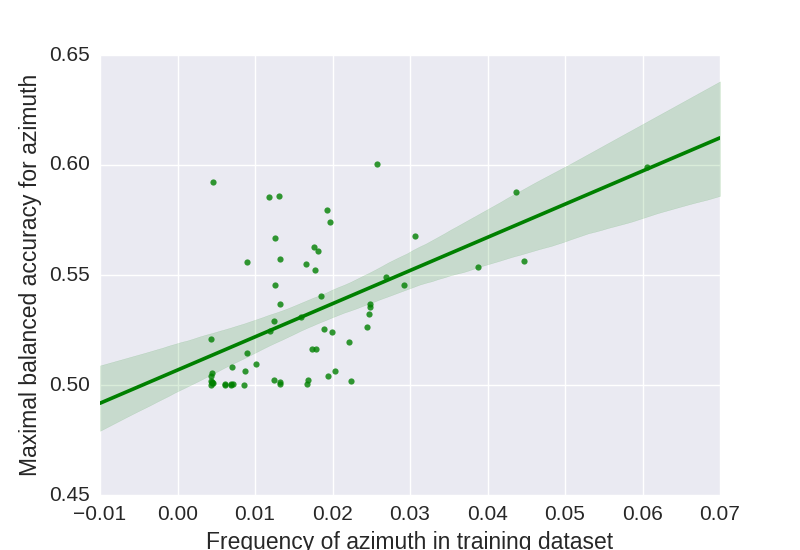
\includegraphics[scale=0.45]{images-data/frequency_accuracy}
\label{fig:results:frequency_accuracy}
\caption{Correlation between the dataset imbalance and the obtained balanced accuracy for each azimuth (regression line and 95\% confidence interval)}
\end{subfigure}
\caption{Results for localization of mixed sounds: balanced accuracy for each azimuth and correlation with localization class percentage ratio}
\end{figure}